\section{Localization and Particle Filter}

To plan how to reach a specific point, the vehicle first has to know \textbf{where it is} in space.
This is the \textbf{localization} problem, and in this chapter we will see what it is, which techniques exist and, in detail, how to solve it with a \textbf{particle filter}.

\subsection{The localization problem}
\begin{wrapfigure}{R}{0.41\textwidth}
    \centering
    \vspace{-10pt}
    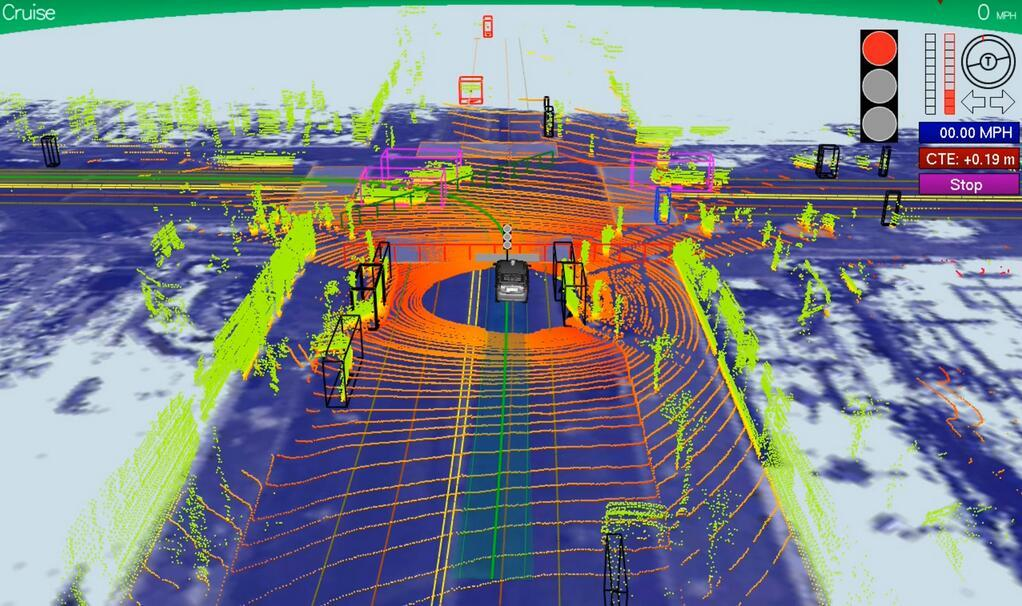
\includegraphics[width=0.4\textwidth]{images/C6_1.png}
    \caption{A vehicle localized in a LiDAR map}
    \vspace{-10pt}
\end{wrapfigure}
Let's suppose we have a car driving on a highway. The traditional way to localize it is the \textbf{GPS}, used to find the car with respect to the map, but the GPS is \textbf{not accurate enough}: it has 2--10\,m of error, while an autonomous car needs something like 2--10\,cm.
Moreover, the GPS signal cannot be guaranteed in occluded areas, such as under trees, in urban canyons (roads surrounded by tall buildings) or in tunnels.
So we cannot trust the GPS alone.

Localization answers the question ``\textbf{where am I?}'', with an accuracy of about \textbf{10\,cm}.
The common practice is to use the onboard sensors (LiDAR, radar) to measure the distance to \textbf{static obstacles} and to compare them with a \textbf{global map}.
To estimate where the car is, we have to \textbf{match the observations with the map}, i.e.\ find the transformation between the local coordinate system of the car and the global coordinate system of the map.

\subsubsection{What each sensor tells us}
\begin{table}[H]
    \centering
    \small
    \begin{tabular}{|l|l|l|p{5.5cm}|}
        \hline
        \textbf{Sensor} & \textbf{Measures} & \textbf{Typical rate} & \textbf{Error behaviour} \\
        \hline
        Wheel odometry & $v$, $\omega$ (relative motion) & 50--100\,Hz & Smooth, drift grows without bound \\
        \hline
        IMU & acceleration, angular rate & 100--1000\,Hz & Bias $\rightarrow$ heading and position drift \\
        \hline
        GNSS & absolute position & 1--10\,Hz & 2--10\,m; lost in tunnels and indoors \\
        \hline
        RTK-GNSS & corrected position & 1--20\,Hz & cm-level in open sky; same outages \\
        \hline
        LiDAR + map & ranges to reflectors & 10--20\,Hz & cm-level; needs a map and data association \\
        \hline
        Camera + map & lanes, signs, features & 30--60\,Hz & Depends on light and weather \\
        \hline
    \end{tabular}
    \caption{What each sensor contributes to localization}
\end{table}

\textbf{Relative} sensors (odometry, IMU) are smooth but they \textbf{drift}; \textbf{absolute} sensors (GNSS, LiDAR or camera with a map) do not drift, but they are noisy or not always available. Localization \textbf{fuses both}.

\noindent\begin{minipage}[c]{0.45\textwidth}
If we had a perfect odometry and a perfect LiDAR, estimating the position of the robot would be easy.
Unfortunately this is unrealistic: both are never perfect, especially the odometry.
With a noisy odometry the error accumulates over time (drift), while with a noisy LiDAR every scan is fuzzy but the error does not grow.
\end{minipage}\hfill
\begin{minipage}[c]{0.51\textwidth}
    \centering
    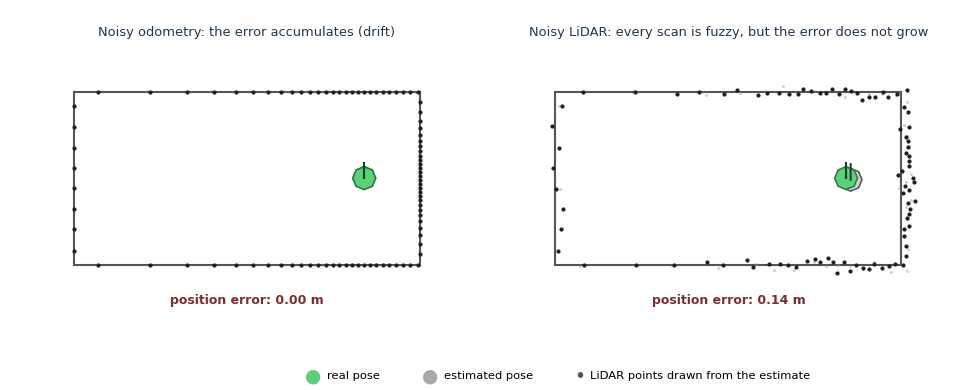
\includegraphics[width=\linewidth]{images/C6_2.png}
    \captionof{figure}{Noisy odometry (left) vs noisy LiDAR (right)}
\end{minipage}

\subsubsection{Localization, mapping and SLAM}
Three related problems must be distinguished:
\begin{table}[H]
    \centering
    \small
    \begin{tabular}{|p{4.6cm}|p{4.6cm}|p{4.6cm}|}
        \hline
        \textbf{Localization} & \textbf{Mapping} & \textbf{SLAM} \\
        \hline
        Given the map $m$, estimate the pose $x_t$ & Given the poses $x_{1:t}$, estimate the map $m$ & Given only controls and measurements, estimate $x_{1:t}$ and $m$ together \\
        \hline
        ``Where am I in this map?'' (this course) & ``What does the world look like?'' & ``Build the map while using it'' \\
        \hline
    \end{tabular}
    \caption{Localization, mapping and SLAM}
\end{table}

Localization itself comes in three problems of increasing difficulty:
\begin{compactitemize}
    \item \textbf{Position tracking}: the initial pose is known with a small uncertainty; a KF, EKF or particle filter is usually enough;
    \item \textbf{Global localization}: the initial pose is unknown, so the belief is \textbf{multimodal} (the robot could be in many places): we need a particle or histogram filter;
    \item \textbf{Kidnapped robot}: the robot is moved without being told; the filter must notice that it is lost and recover.
\end{compactitemize}

\subsection{Landmark-based localization}
\textbf{Localization} is the process of determining the position of a robot within a \textbf{known environment} (a map).
A widely used method is \textbf{landmark-based localization}: the robot identifies \textbf{landmarks}, recognizable features of the environment, and measures its distance from them to estimate its position.
Typical landmarks are road lanes, traffic lights and signals in automotive, or metallic laser reflectors (points with a \textbf{high reflectivity}) in a warehouse.

The map is what makes the difference: without it, dead reckoning causes cumulative errors and the position drifts; with a map, the robot can correct these errors every time it observes known landmarks.

\begin{infobox}[Landmarks or features?]
What Nacho calls \textbf{landmarks}, Davide (who will cover the camera part of the course) will call \textbf{features}: in both cases we mean geometric properties of the environment that we use to understand where we are.
\end{infobox}

\subsubsection{Localization methods}
The localization component estimates the \textbf{pose} of the ego vehicle (position and orientation) relative to a map or to the road.
It is not only based on LiDAR:
\begin{compactitemize}
    \item \textbf{LiDAR-based}: extract road features and compare them with the registered map (this is what we will implement, following Levinson and Thrun, 2010);
    \item \textbf{Camera-based}: based on visual odometry and road maps;
    \item \textbf{LiDAR and camera}: the LiDAR data are used to build the map and the camera to localize the car in it; most of these methods match stereo images to 3D point-cloud maps;
    \item \textbf{GPS}: often combined with LiDAR and cameras for additional global accuracy, especially in open areas where landmarks are sparse.
\end{compactitemize}

\begin{figure}[H]
    \centering
    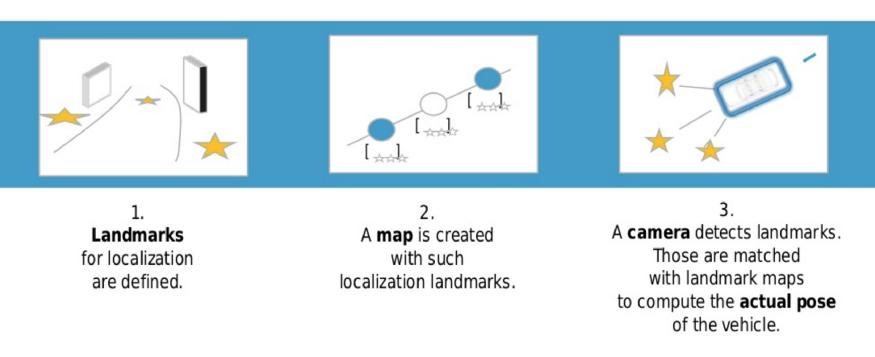
\includegraphics[width=0.6\textwidth]{images/C6_4.png}
    \caption{Landmarks are defined, a map is built with them, and a camera matches them to compute the pose}
\end{figure}

\subsubsection{Dead reckoning}
\noindent\begin{minipage}[c]{0.55\textwidth}
\textbf{Dead reckoning} computes the current position of a moving object from a previously determined position (a \textbf{fix}), integrating the estimates of speed, heading and course over the elapsed time.
For example, wheel encoders count the wheel revolutions to compute how far the vehicle has travelled.
It is useful when the GNSS is not available (e.g.\ in tunnels), but it suffers from the \textbf{drift problem}: an external source is always needed to correct the position.
\end{minipage}\hfill
\begin{minipage}[c]{0.41\textwidth}
    \centering
    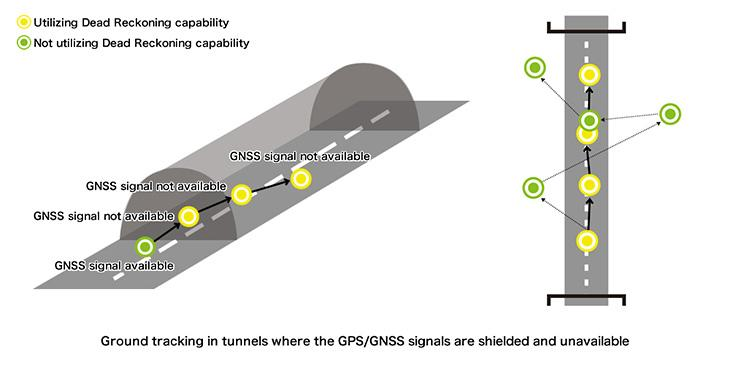
\includegraphics[width=\linewidth]{images/C6_5.png}
    \captionof{figure}{Dead reckoning in a tunnel}
\end{minipage}

\subsection{Mapping}
\noindent\begin{minipage}[c]{0.6\textwidth}
Maps are used to localize the vehicle with \textbf{high precision}.
A \textbf{LiDAR mapping car}, equipped with high-resolution LiDARs, radars, GPS, IMUs and cameras, builds the map \textbf{ahead of time}, with landmarks that are unlikely to change, such as lanes, traffic lights and poles.
The result are \textbf{HD maps}, which contain detailed geometric and semantic information: road shapes, lane configurations and positions of key objects.

\vspace{4pt}Later, a ``cheaper'' vehicle can use the map: it localizes itself by comparing the features of its current measurements with the pre-computed map.
\end{minipage}\hfill
\begin{minipage}[c]{0.36\textwidth}
    \centering
    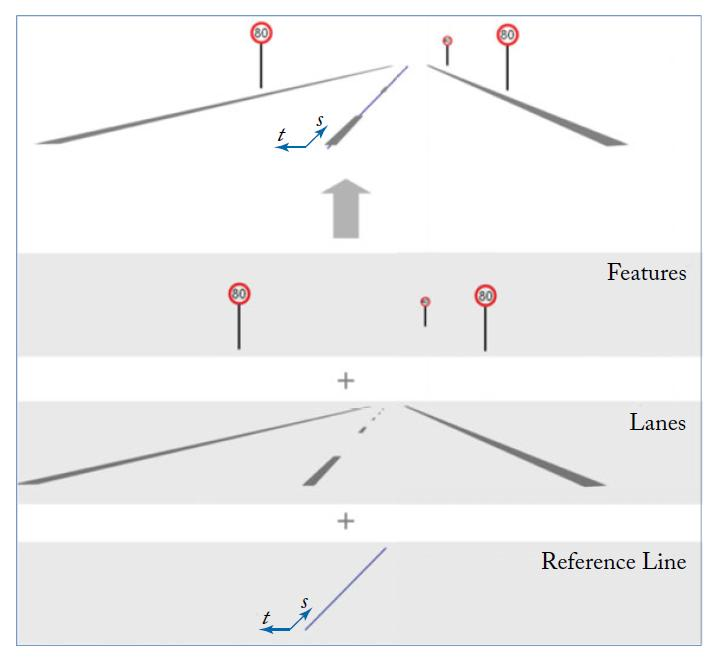
\includegraphics[width=\linewidth]{images/C6_7.png}
    \captionof{figure}{An HD map: features, lanes and reference line}
\end{minipage}

\subsection{SLAM}
If the map does not exist, we can estimate it together with our position: this is \textbf{SLAM} (Simultaneous Localization And Mapping), which builds a map while at the same time estimating the position of the vehicle inside it, using the environment to update the position of the robot.

The \textbf{robot state} is its pose (position and orientation), but it can also include other parameters such as the velocity, the sensor biases and the calibration parameters.
The \textbf{map} contains the aspects of interest of the environment, such as the positions of landmarks and obstacles (a traffic light can be a landmark).

\begin{examplebox}[SLAM as a human visiting a new city]
Imagine visiting a city for the first time:
\begin{compactitemize}
    \item we know how we are moving (\textit{robot: odometry/IMU});
    \item we triangulate our position from things we recognize (\textit{robot: distances to the landmarks}), correcting the accumulated error when we ``open our eyes'';
    \item we update our mental map when we see new things (\textit{robot: add new features to the map});
    \item when we come back to a place we already visited, we understand where we are (\textit{robot: \textbf{loop detection}}, the software detects that the place was already visited, and \textbf{loop closing}, the map is corrected with the gained information).
\end{compactitemize}
\end{examplebox}

\subsubsection{EKF-SLAM}
\noindent\begin{minipage}[c]{0.6\textwidth}
A classical implementation uses an EKF (Extended Kalman Filter), with five steps:
\begin{enumerate}
    \item \textbf{State prediction}: the odometry change updates the predicted pose;
    \item \textbf{Measurement prediction}: where we expect to see the known landmarks;
    \item \textbf{Measurement}: landmarks are extracted from the laser scan;
    \item \textbf{Data association}: the observed landmarks are matched with the known ones;
    \item \textbf{Update}: re-observed landmarks correct the state, new ones are added to it.
\end{enumerate}
\end{minipage}\hfill
\begin{minipage}[c]{0.36\textwidth}
    \centering
    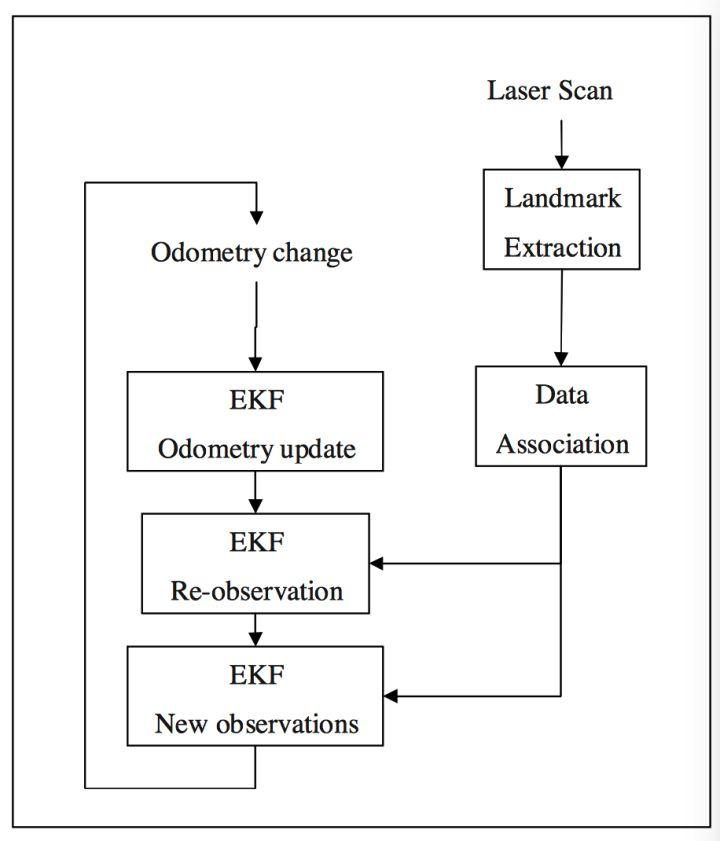
\includegraphics[width=0.85\linewidth]{images/C6_6.png}
    \captionof{figure}{EKF-SLAM}
\end{minipage}

\subsubsection{Front end and back end}
A SLAM system is divided into a \textbf{front end} and a \textbf{back end}.

\begin{figure}[H]
    \centering
    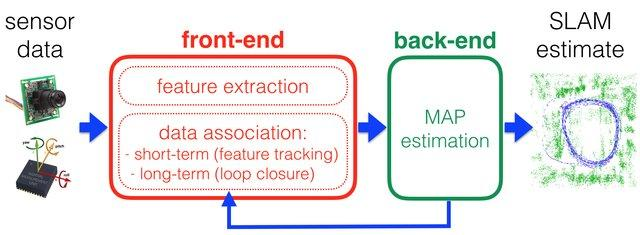
\includegraphics[width=0.55\textwidth]{images/C6_8.png}
    \caption{SLAM front end and back end}
\end{figure}

The \textbf{front end} transforms the sensor information into models that can be used for pose estimation.
In \textbf{vision-based} SLAM it extracts the pixel location of a few distinguishable points (corners, edges, textures): this is \textbf{feature extraction}.
In \textbf{LiDAR-based} SLAM, instead of looking for features, it usually matches whole scans (\textbf{scan matching}, followed by graph optimization).
The front end is also in charge of linking the extracted features to the known landmarks (\textbf{data association}).

The \textbf{back end} processes this information to solve the state estimation problem, i.e.\ to find the pose of the robot and the map. Typical solutions are:
\begin{compactitemize}
    \item \textbf{Kalman filter}: the same technique we used to estimate the state of the other vehicles can define the state of our own vehicle;
    \item \textbf{Particle filter}: a variant of the Bayesian filters that compares the sensor observations with the map, creating particles around the areas where the observations are similar to the map;
    \item \textbf{Graph-based SLAM}: the poses and the measurements are represented as a \textbf{graph}, whose \textbf{nodes} are the states of the robot at different times and whose \textbf{edges} are constraints between states derived from the measurements (odometry, LiDAR scans), acting as ``virtual measurements'' that enforce the consistency of the map.
\end{compactitemize}

\subsubsection{Feature and landmark extraction}
\textbf{Landmarks} are features that can easily be re-observed and distinguished from the environment, and the robot uses them to localize itself. A good landmark must be:
\begin{enumerate}
    \item easily \textbf{re-observable};
    \item \textbf{distinguishable} from the other landmarks;
    \item \textbf{stationary}.
\end{enumerate}

In \textbf{visual SLAM} the classical feature extractors are SIFT (Scale-Invariant Feature Transform), SURF (Speeded Up Robust Features) and ORB (Oriented FAST and Rotated BRIEF).
For \textbf{LiDAR}, two common methods are:

\noindent\begin{minipage}[t]{0.48\textwidth}
\textbf{Spikes}: the algorithm looks for \textbf{extreme differences} between consecutive distance measurements at adjacent angles. A sharp change indicates a geometric change, such as the edge of a wall, a corner or an object boundary, which can be used as a landmark. It fails in smooth environments without sharp changes in geometry.

\vspace{4pt}\centering
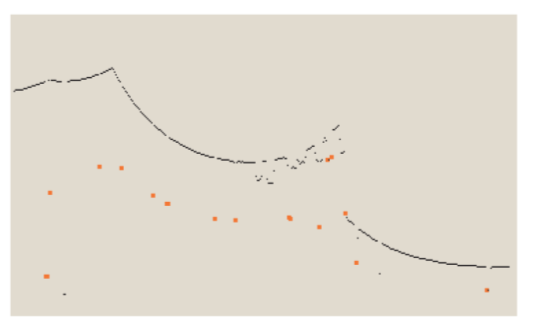
\includegraphics[width=0.85\linewidth]{images/C6_10.png}
\captionof{figure}{Spikes in a laser scan}
\end{minipage}\hfill
\begin{minipage}[t]{0.48\textwidth}
\textbf{RANSAC}: it fits models to the data while filtering out the outliers, and it is used to extract \textbf{lines} from a laser scan (walls, road edges). By matching these lines to the map, or tracking them over time, the robot estimates its position relative to these static features. It fails in cluttered environments.

\vspace{4pt}\centering
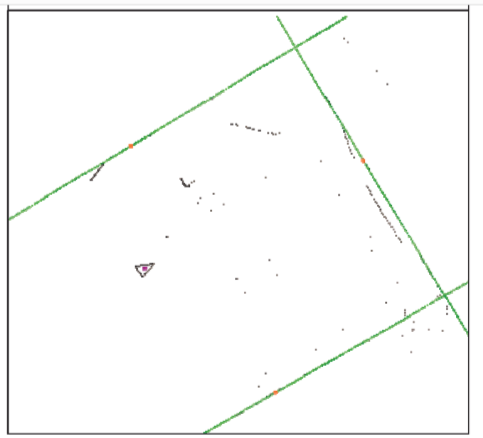
\includegraphics[width=0.6\linewidth]{images/C6_9.png}
\captionof{figure}{Lines extracted with RANSAC}
\end{minipage}

\begin{infobox}[Google vs Tesla]
\textbf{Google (Waymo)} localizes with \textbf{LiDARs}: it relies on all kinds of road features (lane lines, curbs, signals) and on prior \textbf{HD maps}, which are expensive and weak to climate or road changes.
\textbf{Tesla} uses \textbf{vision}: it mostly relies on lane lines and features detected with DNNs. It also uses maps, but less detailed ones (cameras + radars), which is cheap but less accurate. Rather than localizing in the traditional way, Tesla builds a representation of the road geometry on the fly from perception, and the car is inherently localized in it.
\end{infobox}

\subsection{Particle filter}

\subsubsection{From tracking objects to localizing ourselves}
With the Kalman filter we built a tracker for the objects around us. Can we use the same idea to track the \textbf{ego vehicle}, i.e.\ to know where we are in real time?
The two problems look similar, but they are not:

\begin{table}[H]
    \centering
    \small
    \begin{tabular}{|l|p{6.3cm}|p{6.3cm}|}
        \hline
         & \textbf{Object tracking (KF)} & \textbf{Ego localization} \\
        \hline
        State & $[x, y, v_x, v_y]$ of each pedestrian & our pose $[x, y, \theta]$ in a known map \\
        \hline
        Measurement & the cluster centroid, i.e.\ directly a position & LiDAR distances to walls and reflectors, not our position \\
        \hline
        Model & linear $z = Hx$, Gaussian noise & \textbf{nonlinear} $z = h(x, map)$ \\
        \hline
        Belief & one Gaussian per object is enough & may have \textbf{several peaks} \\
        \hline
    \end{tabular}
    \caption{Object tracking vs ego localization}
\end{table}

In localization, before we had the centroids $(x, y)$ of the clusters as measurements, while now we have the \textbf{distances to the objects with high reflectivity}. This brings three problems:
\begin{enumerate}
    \item \textbf{Nonlinear}: a small rotation of the robot changes all the measured distances a lot, while a large translation along parallel walls may produce almost no change;
    \item \textbf{Ambiguous}: symmetric corridors look the same, so the belief has several peaks;
    \item \textbf{Unknown start}: at power-on we could be anywhere in the map.
\end{enumerate}

\begin{figure}[H]
    \centering
    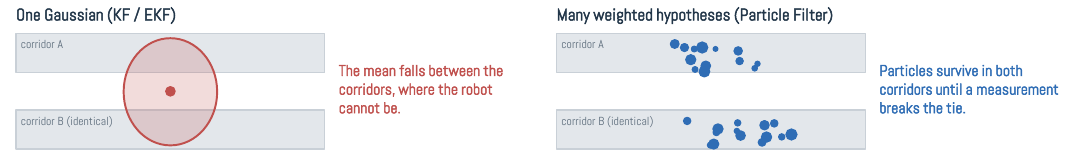
\includegraphics[width=0.75\textwidth]{images/C6_11.png}
    \caption{Two identical corridors: the mean of a single Gaussian falls between them, where the robot cannot be, while particles survive in both until a measurement breaks the tie}
\end{figure}

\subsubsection{When the Kalman filter breaks}
\noindent\begin{minipage}[c]{0.6\textwidth}
Consider a car with a known speed of 10\,m/s and an uncertain heading, $0^\circ \pm 15^\circ$.
After 1\,s the car is always 10\,m away from the start, so the possible positions lie on an \textbf{arc}.
The Kalman filter can only describe the uncertainty as an \textbf{ellipse} (a Gaussian), with a centre and a width: the best ellipse puts its centre at $x = 9.7$\,m, inside the arc, a point where the car can never be, since it always travels 10\,m.
The model \textbf{bends} the uncertainty, and an ellipse cannot bend.
\end{minipage}\hfill
\begin{minipage}[c]{0.36\textwidth}
    \centering
    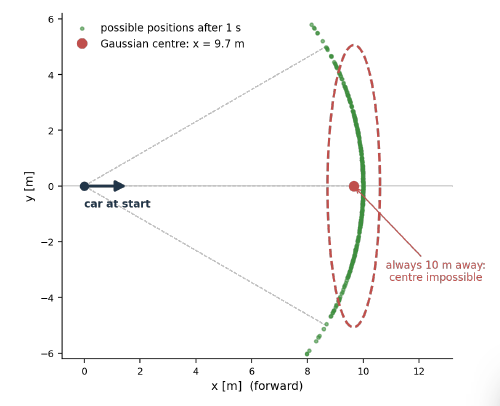
\includegraphics[width=\linewidth]{images/C6_12.png}
    \captionof{figure}{Possible positions (green) vs the Gaussian centre (red)}
\end{minipage}

\vspace{6pt}Is a 30\,cm error really a problem? In one step, no: the problem is what happens next.
The error grows with the \textbf{curvature} and with \textbf{time} ($\pm5^\circ \rightarrow 4$\,cm, $\pm15^\circ \rightarrow 34$\,cm, $\pm30^\circ \rightarrow 1.34$\,m).
Also the uncertainty $P$ is wrong: the filter becomes \textbf{overconfident}, so a measurement saying ``the car is further back'' is almost ignored, and true detections at the ends of the arc may be rejected (wrong gating).
Since the filter is recursive, a wrong state with a too small $P$ can make it \textbf{diverge}.

\paragraph{Solutions: EKF and particle filter}
The \textbf{Extended Kalman Filter} (EKF) pretends the curve is straight: near the current estimate it replaces the curve with its \textbf{tangent} (the derivative, in general the \textbf{Jacobian}, recomputed at every step), and then applies the normal KF.
It is fast (same cost as the KF), but it is wrong when the curvature is high: in our example it puts the centre at $x = 10$\,m with no uncertainty forward (the true one is 0.47\,m), so it is overconfident. Moreover, a Gaussian still cannot represent multimodal uncertainty, like the two corridors.

The \textbf{particle filter} (PF) uses no ellipse at all: it represents the uncertainty with hundreds of \textbf{particles}, each one a possible state, and keeps them as they are.
At every step it moves each particle, weights it (does it agree with the sensor?) and resamples (keeps the good ones).
In this way it keeps the real shape of the belief (a ``banana'', or even two peaks), at the price of being slower, since it needs hundreds or thousands of particles.

\begin{figure}[H]
    \centering
    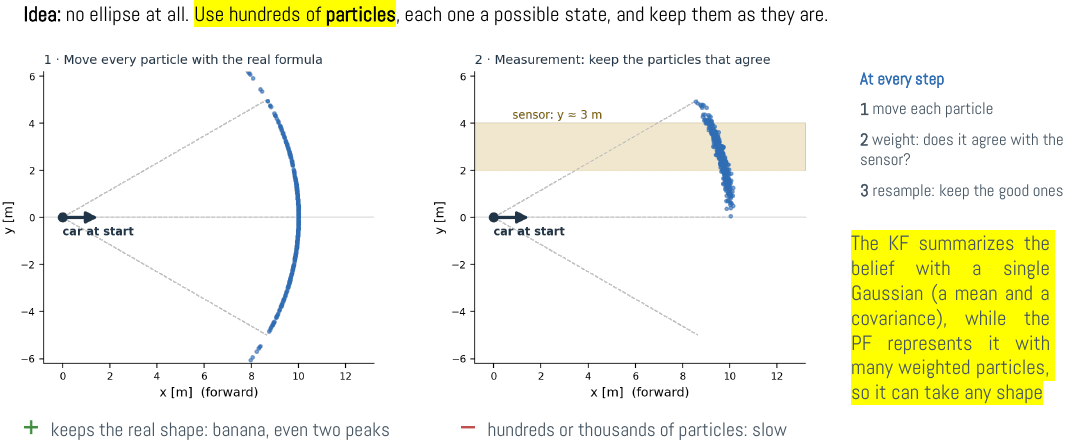
\includegraphics[width=0.8\textwidth]{images/C6_13.png}
    \caption{Particles follow the real arc, and a measurement keeps only those that agree with it}
\end{figure}

\subsubsection{The idea}
A \textbf{particle filter} is a probabilistic estimation technique that represents the probability distribution of the state with a set of \textbf{weighted particles}.
Our objective is to estimate the state $[x, y, \theta]$ of the vehicle, and each particle is a \textbf{discrete hypothesis} (a guess) about it: instead of a single estimate, the filter tracks many possible states, each with a \textbf{weight} proportional to how well it explains the current observations.
We can imagine them as many small Gaussians distributed on the map, each one representing the hypothesis that the robot is in that position.
Like the Kalman filter, it is based on \textbf{Bayesian} logic and it has a very similar structure, but it handles nonlinearity very easily.

\begin{figure}[H]
    \centering
    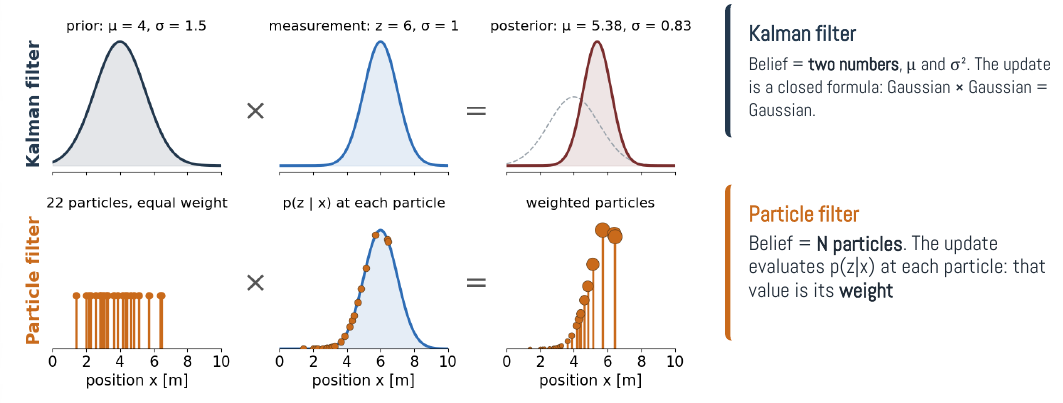
\includegraphics[width=0.75\textwidth]{images/C6_14.png}
    \caption{Same update, two representations: Gaussian $\times$ Gaussian vs weighting each particle with $p(z \mid x)$}
\end{figure}

In the Kalman filter the belief is two numbers, $\mu$ and $\sigma^2$, and the update is a closed formula. In the particle filter the belief is $N$ particles, and the update evaluates $p(z \mid x)$ at each particle: that value is its weight.

\begin{examplebox}[The particle filter in one idea: ask a crowd]
\begin{compactitemize}
    \item ``The vehicle is here'', says one person $\Rightarrow$ a \textbf{particle}: one guess $(x, y, \theta)$;
    \item how much do I trust that person? $\Rightarrow$ its \textbf{weight} $w$;
    \item does the opinion agree with what the sensor sees? $\Rightarrow$ \textbf{update}: $w \propto p(z \mid x)$;
    \item who was wrong copies someone who was right $\Rightarrow$ \textbf{resampling};
    \item the vehicle moves, everyone moves their guess $\Rightarrow$ \textbf{prediction} (motion model).
\end{compactitemize}
\end{examplebox}

\subsubsection{Algorithm}
The input of the algorithm is a \textbf{map} containing the positions of the landmarks (e.g.\ the $(x, y)$ of the reflectors), and we use a LiDAR able to measure the distances to these features.
The algorithm is composed of four steps, the last three repeated at every iteration:
\begin{enumerate}
    \item \textbf{Initialize}: spread the particles;
    \item \textbf{Predict}: move each particle with the motion model (state transition model) of the vehicle, e.g.\ odometry or kinematics, simulating how the vehicle may have moved since the last step;
    \item \textbf{Update}: compare the sensor observations with the map and \textbf{weight} each particle by how well its predicted observations match the real data, i.e.\ how consistent its guessed position is with the real measurements;
    \item \textbf{Resample}: particles with higher weights are more likely to survive, the others are discarded, so the set focuses around the most probable location.
\end{enumerate}

\noindent\begin{minipage}[c]{0.6\textwidth}
\begin{algorithm}[H]
\caption{Particle\_filter$(\mathcal{X}_{t-1}, u_t, z_t)$}
\begin{algorithmic}[1]
    \State $\bar{\mathcal{X}}_t = \mathcal{X}_t = \emptyset$ \Comment{Initialize}
    \For{$m = 1$ to $M$}
        \State sample $x_t^{[m]} \sim p(x_t \mid u_t, x_{t-1}^{[m]})$ \Comment{Prediction}
        \State $w_t^{[m]} = p(z_t \mid x_t^{[m]})$ \Comment{Update}
        \State $\bar{\mathcal{X}}_t = \bar{\mathcal{X}}_t + \langle x_t^{[m]}, w_t^{[m]} \rangle$
    \EndFor
    \For{$m = 1$ to $M$} \Comment{Resampling}
        \State draw $i$ with probability $\propto w_t^{[i]}$
        \State add $x_t^{[i]}$ to $\mathcal{X}_t$
    \EndFor
    \State \Return $\mathcal{X}_t$
\end{algorithmic}
\end{algorithm}
\end{minipage}\hfill
\begin{minipage}[c]{0.36\textwidth}
    \centering
    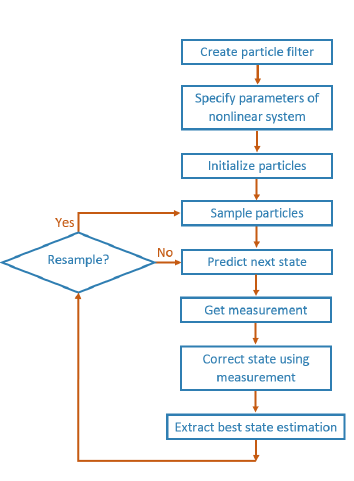
\includegraphics[width=\linewidth]{images/C6_16.png}
    \captionof{figure}{Particle filter flow}
\end{minipage}

\vspace{6pt}At each iteration, every particle $x_{t-1}^{[m]}$ is moved by sampling from the motion model $p(x_t \mid u_t, x_{t-1})$, then it receives the weight $w_t^{[m]} = p(z_t \mid x_t^{[m]})$; finally $M$ particles are drawn with probability proportional to their weights to build the new set $\mathcal{X}_t$.


\begin{table}[H]
    \centering
    \small
    \begin{tabular}{|l|p{11cm}|}
        \hline
        \textbf{Symbol} & \textbf{Meaning} \\
        \hline
        $x_t = (x, y, \theta)$ & pose of the vehicle in the map frame at time $t$ \\
        \hline
        $v$, $\omega$ & linear velocity and yaw rate $\dot{\theta}$ (odometry input $u_t$) \\
        \hline
        $\Delta t$ & time between two odometry messages \\
        \hline
        $z_t$ & measurement: reflectors seen in the vehicle frame \\
        \hline
        $l_j = (l_x, l_y)$ & landmark $j$ of the map $m$ \\
        \hline
        $N$ & number of particles \\
        \hline
        $x^{(i)}$, $w^{(i)}$ & particle $i$ and its weight ($\tilde{w}^{(i)}$ normalized) \\
        \hline
        $\sigma_x$, $\sigma_y$, $\sigma_\theta$ & motion noise (standard deviations) \\
        \hline
        $\sigma_{l_x}$, $\sigma_{l_y}$ & measurement noise (standard deviations) \\
        \hline
    \end{tabular}
    \caption{Glossary of the particle filter}
\end{table}

\subsubsection{Initialization}
The goal of this phase is to generate an \textbf{initial belief} about where the robot might be. Each particle encodes a possible pose $[x, y, \theta]$.
If no prior knowledge is available, the particles are \textbf{uniformly spread} across the map; if an initial guess is available (e.g.\ GPS or a known starting area), they are sampled \textbf{around that estimate} with some noise.
All the particles start with \textbf{equal weights} ($1/N$), representing a uniform belief.

\subsubsection{Map definition}
The map is one of the \textbf{inputs} of the algorithm: it describes the environment and it is the reference for the localization.
It can be built in many ways: with a reflector detection algorithm (if the landmarks are known), with feature extraction from LiDAR or vision data, or with SLAM.
In our case the reflectors have a much higher \textbf{intensity} than the rest of the point cloud: we filter the points by intensity, apply a circle fitting and create the map by clustering the reflectors.

\subsubsection{Prediction}
Where will the vehicle (and the particles) be at the next time step? We need a \textbf{motion model}, a description of the physics of the vehicle, i.e.\ of how it moves at each point in time.
We use the \textbf{CTRV} (Constant Turn Rate and Velocity) model. If the yaw rate $\dot{\theta}$ is 0:
\[
x_f = x_0 + v\,dt \cos\theta_0 \qquad y_f = y_0 + v\,dt \sin\theta_0 \qquad \theta_f = \theta_0
\]
otherwise:
\[
\begin{aligned}
x_f &= x_0 + \frac{v}{\dot{\theta}}\left[\sin(\theta_0 + \dot{\theta}\,dt) - \sin\theta_0\right] \\
y_f &= y_0 + \frac{v}{\dot{\theta}}\left[\cos\theta_0 - \cos(\theta_0 + \dot{\theta}\,dt)\right] \\
\theta_f &= \theta_0 + \dot{\theta}\,dt
\end{aligned}
\]
where $x_0$ is the initial position, $x_f$ the final one and $dt$ the elapsed time.
Every particle is moved with this model, plus some random noise ($\sigma_x$, $\sigma_y$, $\sigma_\theta$).

\subsubsection{Update}
Each particle carries a \textbf{weight} that indicates how likely it is to correspond to the true position of the vehicle.
The weight is computed by comparing the measurements \textbf{predicted} from the pose of the particle with the \textbf{actual} sensor observations: the closer they are, the larger the weight and the more important the particle.
The particle with the maximum weight represents the best estimate of the position.

\noindent\begin{minipage}[c]{0.5\textwidth}
For example, the map contains the landmarks $L_1$, $L_2$, $L_3$ and the sensor of the real vehicle (whose position the filter does not know) measures $Z = (4.24, 5.83, 4.47)$\,m.
For each particle we compute the distances $\hat{z}$ it would measure if it were the vehicle. Which particle should we trust more? The weight answers this question.
\end{minipage}\hfill
\begin{minipage}[c]{0.46\textwidth}
    \centering
    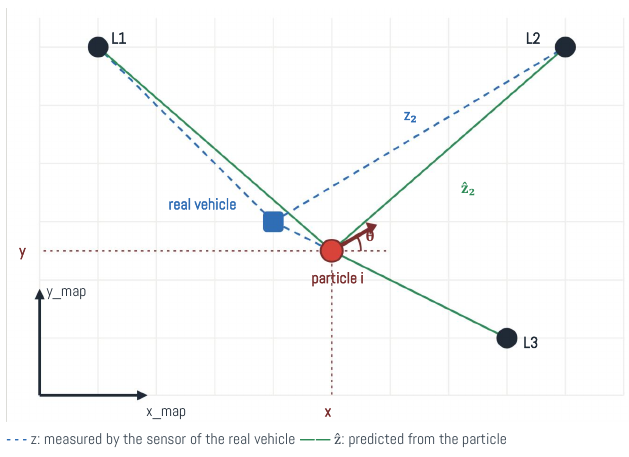
\includegraphics[width=\linewidth]{images/C6_18.png}
    \captionof{figure}{Measured $z$ (dashed) vs predicted $\hat{z}$ (green)}
\end{minipage}

\vspace{6pt}\noindent\begin{minipage}[c]{0.5\textwidth}
In practice, for each landmark $j$ we take the gap $e_j = z_j - \hat{z}_j$ between the measured and the predicted distance and score it with a Gaussian; the weight is the \textbf{product} over all the landmarks:
\[
w = \prod_j \mathcal{N}(z_j;\ \hat{z}_j,\ \sigma^2)
\]
If we project each measured distance onto the particle, for a good particle the segment ends almost exactly on the landmark: small gaps, large weight.
\end{minipage}\hfill
\begin{minipage}[c]{0.46\textwidth}
    \centering
    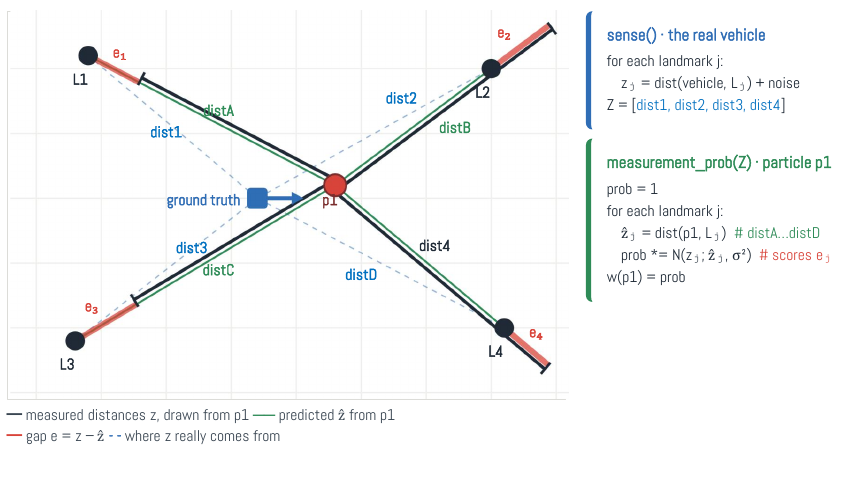
\includegraphics[width=\linewidth]{images/C6_19.png}
    \captionof{figure}{Gaps $e_j$ (red) between measured and predicted distances}
\end{minipage}

\vspace{6pt}\noindent\begin{minipage}[c]{0.5\textwidth}
Why a Gaussian? Because the \textbf{sensor makes errors}: if we measure the same reflector many times, the readings are never exactly the same and they form a bell centred on the true distance, whose width $\sigma$ is the typical error of the sensor. This bell is exactly the measurement noise $R = \sigma^2$ of the Kalman filter.
If the particle were the vehicle, the gap $e_j$ would just be a sensor error, and the height of the bell at $e_j$ says how common that error is: that becomes the weight.
\end{minipage}\hfill
\begin{minipage}[c]{0.4\textwidth}
    \centering
    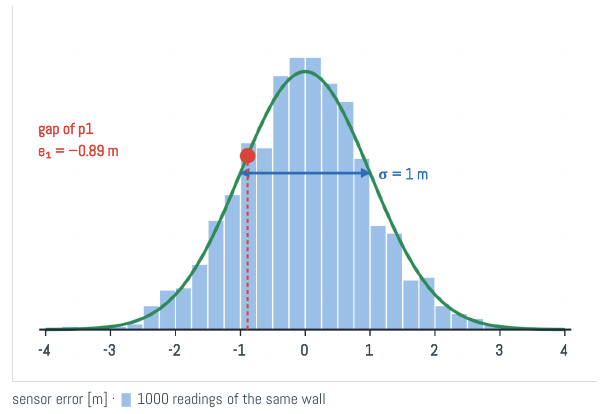
\includegraphics[width=\linewidth]{images/C6_20.png}
    \captionof{figure}{1000 readings of the same wall ($\sigma = 1$\,m)}
\end{minipage}

\begin{examplebox}[Weight of two particles]
With $\sigma = 1$\,m and 4 landmarks, particle $p_1$ (1.22\,m from the real vehicle) has gaps $e = (-0.89, +1.12, -1.10, +0.89)$\,m, which give $\mathcal{N} = 0.269, 0.213, 0.217, 0.269$, so
\[
w(p_1) = 0.269 \cdot 0.213 \cdot 0.217 \cdot 0.269 = 0.0033
\]
Particle $p_2$ (only 0.28\,m away) has all gaps below 0.3\,m: $\mathcal{N} = 0.399, 0.385, 0.384, 0.398$, so $w(p_2) = 0.0234$.
A particle exactly on the vehicle would get $0.399^4 = 0.0253$: $p_1$ has about 13\% of it, $p_2$ about 92\%.
\end{examplebox}

\begin{figure}[H]
    \centering
    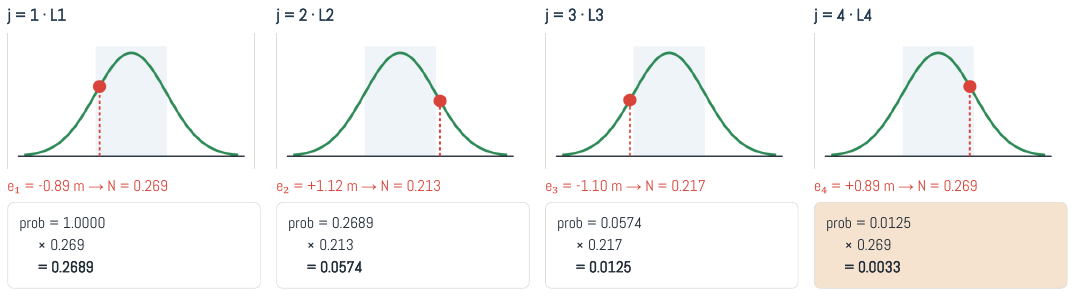
\includegraphics[width=0.8\textwidth]{images/C6_21.png}
    \caption{Weight of $p_1$: each gap is scored on the bell and the results are multiplied}
\end{figure}

\begin{infobox}[Data association]
In this example we know that \texttt{dist1} belongs to $L_1$. In reality, when we measure the distances to the reflectors we do not know \textbf{which landmark} each measurement belongs to: the reflectors have no label.
So, before computing the weights, we have to \textbf{associate} each observation to a landmark of the map (after transforming it into map coordinates).
\end{infobox}

\paragraph{Importance weight}
Summing up, \texttt{measurement\_prob} computes how likely a measurement is: the Euclidean distance compares predicted and actual readings, the Gaussian measures how far the prediction is from the real measurement, and the resulting probabilities are the \textbf{importance weights} of the particles.
Then we let the important particles survive \textbf{at random}, with a probability proportional to their weight, and we generate the new particles: this is the \textbf{resampling}.

\begin{lstlisting}
def measurement_prob(self, measurement):
    prob = 1.0
    for i in range(len(landmarks)):
        dist = sqrt((self.x - landmarks[i][0]) ** 2 + (self.y - landmarks[i][1]) ** 2)
        prob *= self.Gaussian(dist, self.sense_noise, measurement[i])
    return prob
\end{lstlisting}

\subsubsection{Resampling}
\noindent\begin{minipage}[c]{0.5\textwidth}
The raw weights are \textbf{not probabilities}: $\mathcal{N}$ is a probability \emph{density}, whose peak is $1/(\sqrt{2\pi}\sigma) = 0.399$ for $\sigma = 1$\,m (and 2 for $\sigma = 0.2$\,m), so even a perfect particle gets $0.399^4 = 0.025$ with 4 landmarks.
So first we \textbf{normalize} them, $\tilde{w} = w / \sum w$, so that they sum to 1.
In the example, $\sum w = 0.0033 + 0.0234 = 0.0267$, so $\tilde{w}(p_1) = 0.13$ and $\tilde{w}(p_2) = 0.87$.
$\tilde{w}$ is the probability that a particle is copied: resampling 10 particles we get on average 1.3 copies of $p_1$ and 8.7 of $p_2$, so $p_2$ survives and multiplies, while $p_1$ tends to disappear.
\end{minipage}\hfill
\begin{minipage}[c]{0.45\textwidth}
    \centering
    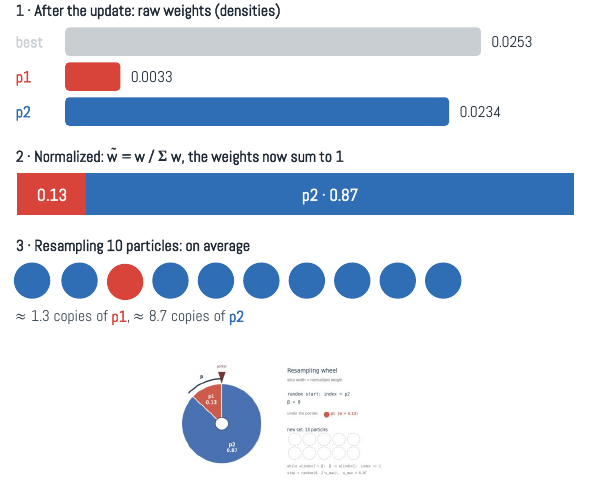
\includegraphics[width=\linewidth]{images/C6_22.png}
    \captionof{figure}{Raw weights, normalized weights and resampling}
\end{minipage}

\vspace{6pt}During the resampling, particles are drawn randomly with a probability proportional to their weight: this removes the unlikely particles and duplicates the more probable ones. There are many resampling algorithms; a simple one is:
\begin{enumerate}
    \item sample $N$ particles with their weights;
    \item normalize the weights;
    \item replace the low-weight particles, drawing new particles from the old ones \textbf{with replacement}, in proportion to the importance weights.
\end{enumerate}

\begin{examplebox}[Normalizing the weights]
With $N = 6$ particles of weights $1.4, 0.5, 0.9, 3.2, 1.9, 0.1$ we have $\sum w_i = 8$, so the probabilities of being drawn are
$\alpha = 0.175,\ 0.0625,\ 0.1125,\ 0.4,\ 0.2375,\ 0.0125$.
\end{examplebox}

\paragraph{Resampling wheel}
\noindent\begin{minipage}[c]{0.6\textwidth}
The \textbf{resampling wheel} is a common way to implement it. Each particle occupies a slice of a wheel proportional to its weight:
\begin{enumerate}
    \item pick a random starting index and set $\beta = 0$;
    \item for each new particle, add to $\beta$ a random value between 0 and $2 \cdot w_{max}$;
    \item while the weight of the current particle is smaller than $\beta$, subtract it from $\beta$ and move the index to the next particle;
    \item when it is bigger, take that particle.
\end{enumerate}
\end{minipage}\hfill
\begin{minipage}[c]{0.4\textwidth}
    \centering
    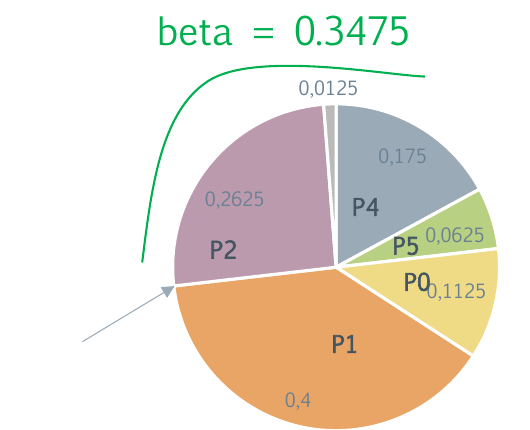
\includegraphics[width=\linewidth]{images/C6_23.png}
    \captionof{figure}{$\beta$ slides along the wheel}
\end{minipage}

\begin{lstlisting}
particles = []
index = int(random.random() * NumParticles)
beta = 0.0
maxWeight = max(weight)
for i in range(NumParticles):
    beta = beta + random.random() * 2 * maxWeight
    while weight[index] < beta:
        beta = beta - weight[index]
        index = (index + 1) % NumParticles
    particles.append(p[index])
\end{lstlisting}

$\beta$ is like a pointer that slides along the wheel: each time we push it forward by a random value between 0 and $2\,w_{max}$, so sometimes we make big jumps (favouring heavier particles), other times small jumps (giving lighter particles a chance too).
At the end each particle is picked in proportion to its slice of the circumference.
If we used only \texttt{random.random() * maxWeight}, the step would always be in $[0, w_{max}]$ and we would be too biased towards the particles with weights close to $w_{max}$.

\paragraph{Other resampling methods}
In \textbf{systematic resampling} we use a single random number: the wheel has $N$ \textbf{evenly spaced} pointers, shifted by one random offset, and each pointer selects a particle.
\textbf{Stratified resampling} is the same, except that the pointers are not evenly placed: each one is drawn randomly inside its own interval of size $1/N$.

\begin{figure}[H]
    \centering
    \begin{subfigure}{0.2\textwidth}
        \centering
        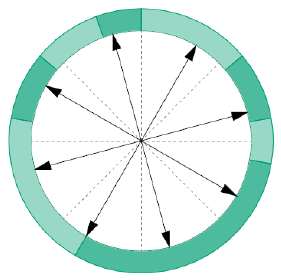
\includegraphics[width=\linewidth]{images/C6_25a.png}
        \caption{Systematic}
    \end{subfigure}
    \hspace{1.5cm}
    \begin{subfigure}{0.2\textwidth}
        \centering
        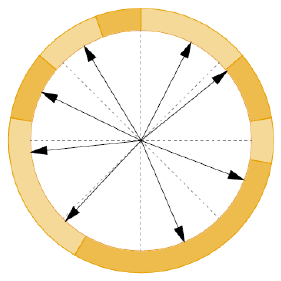
\includegraphics[width=\linewidth]{images/C6_25b.png}
        \caption{Stratified}
    \end{subfigure}
    \caption{Pointers of systematic and stratified resampling}
\end{figure}

\begin{table}[H]
    \centering
    \small
    \begin{tabular}{|l|c|c|c|p{5cm}|}
        \hline
        \textbf{Method} & \textbf{Random numbers} & \textbf{Cost} & \textbf{Variance} & \textbf{Idea} \\
        \hline
        Multinomial & $N$ & $O(N \log N)$ & highest & $N$ i.i.d.\ draws, binary search on the CDF \\
        \hline
        Wheel & $N$ & $\sim O(N)$ & $\approx$ multinomial & heuristic walk, easy to code \\
        \hline
        Stratified & $N$ & $O(N)$ & lower & one draw in each $1/N$ stratum \\
        \hline
        Systematic & 1 & $O(N)$ & lowest in practice & evenly spaced pointers, one offset \\
        \hline
        Residual & $\leq N$ & $O(N)$ & low & copy $\lfloor N\alpha \rfloor$ deterministically, resample the rest \\
        \hline
    \end{tabular}
    \caption{Resampling methods at a glance}
\end{table}

\paragraph{Limitations of resampling}
Resampling only by weight has \textbf{no exploration}: the high-weight particles dominate, and over time most particles become identical (\textbf{particle degeneracy}).
Moreover, even the best particles are only an approximation of the true state: without noise, the filter quickly loses diversity (\textbf{particle impoverishment}).
For this reason we add a \textbf{small random noise} to the particles during the resampling: the new particles are sampled \textbf{around} the best estimates, which refines the estimate by exploring the states close to the best particles and avoids premature convergence to a suboptimal state.

\subsubsection{Recovering when lost: random particle injection}
If the measurements suddenly stop matching, the filter is \textbf{lost}: for example the robot has been moved (kidnapped robot), no particle is close to it, and after the resampling the cloud is compact but in the wrong place.

\begin{figure}[H]
    \centering
    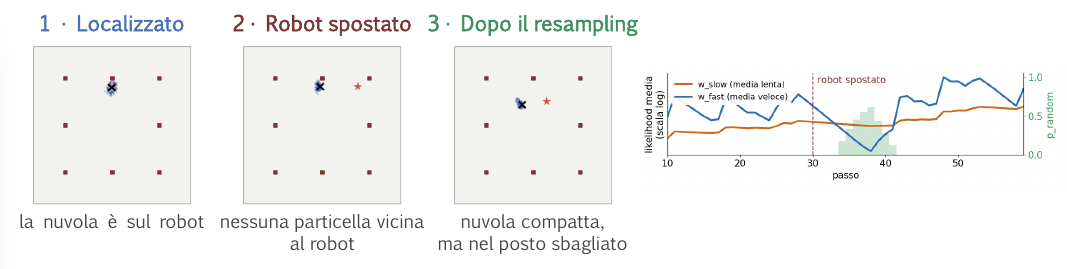
\includegraphics[width=0.75\textwidth]{images/C6_26.png}
    \caption{Localized, robot moved, compact cloud in the wrong place}
\end{figure}

We can detect it by comparing two averages of the likelihood, a slow one and a fast one, and react by \textbf{injecting random particles} (\textbf{Augmented MCL}).
$w_{avg}$ is the mean of the unnormalized weights, i.e.\ how well the particles explain the measurement now; its ``normal'' value depends on the visible landmarks and on the noise, so we cannot use a fixed threshold.
Instead we keep a long-memory average $w_{slow}$ (roughly the last 1000 steps: like the average grade of the year) and a short-memory one $w_{fast}$ (roughly the last 10 steps: the average grade of the week):
\begin{lstlisting}
w_avg  = mean of the unnormalized weights
w_slow += alpha_slow * (w_avg - w_slow)     # e.g. alpha_slow = 0.001
w_fast += alpha_fast * (w_avg - w_fast)     # e.g. alpha_fast = 0.1
for each new particle:
    if rand() < max(0, 1 - w_fast / w_slow):
        add a random pose in the free map
    else:
        draw from the weights
\end{lstlisting}
When the recent likelihood drops below the usual one ($w_{fast} < w_{slow}$), a fraction of the particles is replaced by random poses, so that the filter can find the robot again.

\subsubsection{Kalman filter vs particle filter}
\begin{figure}[H]
    \centering
    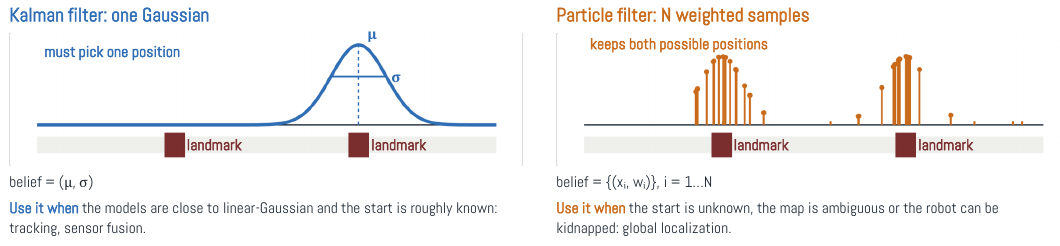
\includegraphics[width=0.75\textwidth]{images/C6_27.png}
    \caption{One Gaussian must pick one position, $N$ weighted samples keep both}
\end{figure}

\begin{table}[H]
    \centering
    \small
    \begin{tabular}{|l|p{5.5cm}|p{5.5cm}|}
        \hline
         & \textbf{Kalman filter (KF / EKF)} & \textbf{Particle filter} \\
        \hline
        Belief & $(\mu, \sigma)$ & $\{(x_i, w_i)\},\ i = 1 \dots N$ \\
        \hline
        Models & linear + Gaussian (EKF: linearized) & any motion and sensor model \\
        \hline
        Belief shape & one peak only & any shape, several peaks \\
        \hline
        Global localization, kidnapping & needs a good initial guess & start anywhere, recover \\
        \hline
        Cost & tiny: a few matrices & $N$ particles $\times$ $M$ observations \\
        \hline
        When the model fits & optimal, smooth estimate & approximate, noisy with few particles \\
        \hline
    \end{tabular}
    \caption{KF vs PF}
\end{table}

Use the \textbf{Kalman filter} when the models are close to linear-Gaussian and the start is roughly known (tracking, sensor fusion); use the \textbf{particle filter} when the start is unknown, the map is ambiguous or the robot can be kidnapped (global localization).
